
%\newpage
\section{Selftest Function}
\label{sec:selftest}
Beginning with release 0.9k I have implemented a self test function. Usage is very simple.
If you have installed  test terminal with clamps, put all clamps together to a piece of uninsulated wire and press the start button.
The program notice the shorten probes and start the self test function, if you confirm within two
seconds with pressing the start key. This confirmation is implemented to prevent the tester
going automatically to the self test by connecting a defect transistor.
After finishing the self test the transistor tester will continue with normal measurement.
If no equipment is connected, the program will end with ``part unknown or damaged''. 
You can configure self test only for a ATmega168  or ATmega328.
Before the test steps begin, the zero resistance of the connected probes is determined for all three combinations
(T1:T3, T2:T3 and T1:T2).
This zero resistances will be subtracted for the future ESR and resistance measurements below \(10\Omega\).
Only zero resistance values below \(0.90\Omega\) are accepted, because this correction values are not
uses for measurement of resistor values above \(10\Omega\).
If you use cables for measurement, you should only take cables with low resistance values.
If the later measured resistance results fall below the particular zero resistance for more than \(0.2\Omega\),
the tester will be resetted to ''uncalibrated''.
This will be marked by a acticated cursor during the tests.
The separate steps of the self test function 1 to 7 is displayed on row~1 of the LCD display with the letter T
followed by the step number.
Every step is repeated 4~times, before the program continues with the next step.
But if you hold the start key pressed, when the test cycle is finished, this test is not repeated any more.
If you leave the key pressed the total time, every test is executed only once.

Without the AUTO\_CAL option only measurement results are displayed in every step, no error analysis are done, you must interpret the results yourself.
At this place I will give you an additional important hint. Never do a measurement with connected ISP plug!
The ISP interface influences the measurement. 
\vspace{1cm}
Here is the list of currently implemented tests:
\vspace{1cm}
\begin{enumerate}
\item {\bf Measurement of the \(1.3V\) (or \(1.1V\)) reference Voltage (band gap Reference).}
In row 1 the text ``Ref='' and the measured Voltage in mV is displayed.
For the ATmega8 the voltage should be near to \(1.3V\). For the other processors the voltage should be near to \(1.1V\).
The second row shows the resulting factor for the capacity measurement with the \(470k\Omega\) resistor.
\item {\bf Comparing of the  \(680\Omega\) resistors.}
In row~1 the cryptic text  ``+RL- 12 13 23'' is shown. Meaning of this is as follows: 
The RL is the short form of Resistor Low meaning the \(680\Omega\) resistors. The 12 stand for: 
resistor at pin~1 is connected to VCC (+) and resistor at pin~2 is connected to GND (-). 
The result of this measurement  is displayed in row~2 at the first place as difference to the theoretical value. 
 In row~1 follows now a ``13'' which means, that the first connection of measurement~1 is still connected
with \(680\Omega\) to VCC but that the resistor of pin~3 is connected to GND.
The result is displayed in the middle place of row~2 as difference to the theoretical value. 
The last measurement of this test ``23.'' means that now the resistor at pin~2 is connected to VCC (+) and
the resistor of pin 3 is connected to GND.
The result of measurement is displayed at the last place of LCR row~2 as difference to the theoretical value.
Please remember, that the resolution of the ADC is about \(4.88mV\)!
The measurement situation is also shown in figure~\ref{fig:test2}.
The theoretical value with respect to the internal resistance of the pins should be: 
\(\frac{5001 \cdot  (19+680)}{ (19+680+680+22)} = 2493\) .

\begin{figure}[H]
\centering
 \begin{overpic}[width=17cm]{../FIG/Test2.pdf}
  \color{black}
  \put(18,22){\makebox(0,0)[cb]{first measurement}}
  \put(49,22){\makebox(0,0)[cb]{second measurement}}
  \put(85,22){\makebox(0,0)[cb]{third measurement}}
 \end{overpic}
\caption{Comparison of \(680\Omega\) resistors }
\label{fig:test2}
\end{figure}

\item {\bf Comparing of the \(470k\Omega\) resistors.}
Now the display shows in row 1 ``+RH- 12 13 23''. The same procedure as done in step~2 is repeated with the \(470k\Omega\) resistors (symbols RH).
All results are shown as difference to the theoretical value.
The theoretical value is this time \(\frac{5001 \cdot (19 + 470000]}{ (19 + 470000 + 470000 + 22)} = 2500\) for all combinations.

\item In this step nothing is measured, but the {\bf order is displayed „ isolate Probe!“},
which means that it is time to separate the probes (release from wire).
This step will finish only if you release the connections between the probes.

\item {\bf This step tests the capability of GND (-) connected \(470k\Omega\) resistors (H) to pull the test pins to GND.}
Row 1 shows the text  ``RH-''.
Row 2 should display zero for all three pins.

\item {\bf This step tests the capability of VCC (+) connected \(470k\Omega\) resistors (H) to pull the test pins  to VCC (+).}
Row 1 shows the text ``RH+''.
The results are shown als difference to VCC and should be near zero.
 Great differences from the best value for test 5 and 6 are errors  such as isolation problem, flux material or damaged port.

\item {\bf This Step tests the voltages of the \(470k\Omega / 680\Omega\)  resistor divider.}
The voltage difference to the expected voltage of the \(470k\Omega\) / \(680\Omega\) resistor dividers is shown
in row 2 of the LCD for all three terminals.
Differences of more than some mV can be caused by the assembly of wrong resistor values.

\item {\bf Measuring of internal resistance of pin output switched to the GND signal.}
This test and the follwing tests will only be done, if the option AUTO\_CAL is selected.
The internal resistance of the port C outputs switched to GND (-) are measured with the current
of to VCC (+) switched \(680\Omega\) resistors, see Figure~\ref{fig:test7}.
Only the three pins of the ADC port are measured, the resistor port B (PB0,PB2 and PB4) can not be measured
without hardware modification.
Is is assumed that the port resistance of the different ports are nearly identical.
The resistor value will be shown in the next test.
\begin{figure}[H]
\centering
 \begin{overpic}[width=15cm]{../FIG/Test7.pdf}
  \color{black}
  \put(16,34){\makebox(0,0)[cb]{first measurement}}
  \put(47,35){\makebox(0,0)[cb]{second measurement}}
  \put(84,35){\makebox(0,0)[cb]{third measurement}}
 \end{overpic}
\caption{Measurement of internal resistance of Port C switched to GND }
\label{fig:test7}
\end{figure}

\item {\bf Measuring of internal resistance of port outputs switched to the VCC (+)signal.}
The needed current is generated with to GND connected \(680\Omega\) resistors .
It are the same measurements as those in test~8 to the other side as you can see in Figure \ref{fig:test8}.
With the following steps the resistance is computed:
To get the current, the following is computed:  \((VCC - (result of test 8) - (result of test 9)) / 680\).
To get both resistor values, the voltage (result of test~8 or 9) is divided by this current.
The result for this test will then be notified in row 1 with the text ''RI\_Hi='', the resistance value (\(\Omega\)) to the GND side is
displayed in row 2 with the text ''RI\_Lo=''.
Beginning with version 1.06k of the software, the port output resistance values are determined at the beginning of every
measurement. The values are only shown by this step.

\begin{figure}[H]
\centering
 \begin{overpic}[width=15cm]{../FIG/Test8.pdf}
  \color{black}
  \put(16,35){\makebox(0,0)[cb]{first measurement}}
  \put(47,35){\makebox(0,0)[cb]{second measurement}}
  \put(84,35){\makebox(0,0)[cb]{third measurement}}
 \end{overpic}
\caption{Measurement of internal resistance of Port C switched to VCC }
\label{fig:test8}
\end{figure}

\item {\bf Measurement of the zero offset of the capacitor measurement.}
The zero offset for the capacity measurement with pin combinations 1:3, 2:3 and 1:2 is shown in that order
in display row 1 following the ``C0 ''.
Alls three values are shown in pF units.
For this measurements no predefined zero offset is respected.
The zero offsets of pin combinations in opposite order is also measured.
The results will be written to the EEprom, if all values are less than \(190pF\).
This will be notified by the output of ``OK'' in row~2.
The found zero offsets are used for further capacity measurements with respect to the pin combination.
If there is any measurement found with a capacity value \(20pF\) below the particular zero offset, the
tester will be resetted to ''uncalibrated''.
This will be noticed by a activated LCD cursor during further tests.
Please notice, that changes of the test equipment can cause a new adjustment of the zero offset.
If you use wire with clips, the zero offset may be \(3pF\) greater compared to a empty socket.

If the tester is configured with the SamplingADC function, the zero capacity values is determined
with double the count of all pin combinations. The reason for this is, that the
zero capacity is measured for the charge and the discharge of all pin combinations separately.

\item {\bf Wait for the connection of a capacitor to pin~1 and pin~3.}
The message ``\mbox{\begin{large}1 \electricC 3~\textgreater 100nF\end{large}}'' is shown in row 1 of LCD.
To prepare the measurement of the comparator offset voltage, you must connect
a sufficient big capacitor to pin~1 and pin~3.
It should be a capacitor with a high quality factor and a capacity between \(100nF\) and \(20\mu F\).
You should never use electrolytical capacitors, use film capacitors instead.

\item {\bf Measurement of the comparator offset for capacitor measurement adjustment.}
To get the offset of the analog comparator, a capacitor must already be connected to pin~1 and pin~3.
The capacitor is needed for buffering the load voltage of a capacitor, in order to get the voltage
difference of load voltage to the internal reference voltage (band gap).
If measurement is successfull, the correction value is short shown with the text ``REF\_C='' in row~1 of 
the LCD and written to the EEprom. You can give a additional offset to the automatic measured value
with the REF\_C\_KORR option.

If you have selected the AUTOSCALE\_ADC option, the gain of the ADC readings with the internal reference
will be adjusted by comparing a capacitor voltage below 1 V once readed with VCC reference and once
readed with the internal reference. 
The measurement result is shown in row 2 with the text ``REF\_R=''. 
Your REF\_R\_KORR value is a additional offset to this automatic find out difference value.

\item {\bf Wait for a capacitor for measuring of low inductace values}
If the tester is configured with the SamplingADC function, a known capacitor is required for
the computation of the inductance value from the resonant frequency of a parallel connected coil.
Practical capacity values can be choosed from \(10nF\) to \(27nF\). 
A suitable capacitor must be connected to pin~1 and pin~3, if the message ''\mbox{\begin{large}1 \electricC 3~10-30nF(L)\end{large}}'' is shown in
line 1 of the display.
Exacly this capacitor should be connected later parallel to a little coil,
if the calculation of the coil\'s inductance value from resonant frequency is desired.
If your tester does not include the SamplingADC function, this step is omitted.

\end{enumerate}

At the end of test function the text ``Test End''  is shown in row~1 and the version number of software is shown in row~2.
If the Makefile option FREQUENCY\_50HZ is set, a {\bf 50Hz rectangle signal} is generated on pin~2 and 
the same signal in opposite direction on pin~3.
Pin~1 is switched to GND . The current is limited with \(680\Omega\) resistors.
This will be notified by the Output of ``50Hz'' at the end of row 1 of the LCD display.
The \(50Hz\) signal will be generated 30 times for 2~seconds each.
You can check the time of the wait calls, if you have an oscilloscope or frequency counter.
Figure \ref{fig:Frequency50} shows the oscillograph curves of both \(50Hz\) output pins with crystal operation.

\begin{figure}[H]
\centering
\includegraphics[]{../PNG/Frequency50.png}
\caption{Oscillograph curve with the 50Hz outputs of Port 2 and 3}
\label{fig:Frequency50}
\end{figure}


If you don't use the crystal clock version, the result may be inexactly.
A exactly clock frequency and wait time are important for measurement of capacity values.
You can abort the generation of the \(50Hz\) signal by long time pressing of the start button.
Then the program continues with the normal measurement task.

\subsection{Some Results of the Selftest Function}

The results of the selftests of nine different ATmega168 processors and of six ATmega328 processors
will be shown in the following figures.

\begin{table}[H]
  \begin{center}
    \begin{tabular}{| l | c | c | c |}
    \hline
Test No. & measurement typ & theoretical & figure \\
    \hline
    \hline
Test 1 & band gap Ref  & 1100 & \ref{fig:SelfTref} \\
    \hline
Test 2 & RL-Mean & 0 & \ref{fig:SelfTMitL} \\
    \hline
Test 3 & RH-Mean & 0 & \ref{fig:SelfTMitH} \\
    \hline
Test 5 & RH-Low &  0 & \ref{fig:SelfTlowH} \\
    \hline
Test 6 & RH-High & 0 & \ref{fig:SelfTtopH} \\
    \hline
Test 8 & R out Lo & 131 & \ref{fig:SelfTRoL} \\
    \hline
Test 9 & R out Hi & 151 & \ref{fig:SelfTRoH} \\
    \hline
Test 10 & Cap zero offset & 30 & \ref{fig:SelfTcap} \\
    \hline
Test 11 & Reference correction & 0 & \ref{fig:SelfTrefKorr} \\
    \hline
    \end{tabular}
  \end{center}
  \caption{Table of the selftest figures }
  \label{tab:test_m168} 
\end{table}

\begin{figure}[H]
\centering
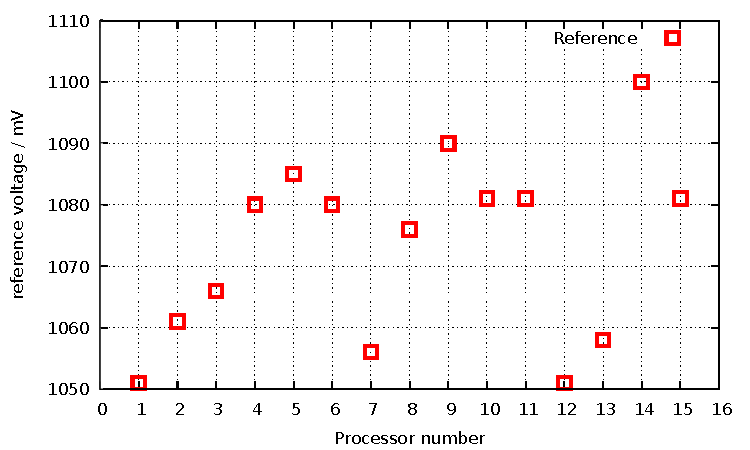
\includegraphics[width=16cm]{../GNU/SelfTref.pdf}
\caption{Selftest: Reference-Voltages}
\label{fig:SelfTref}
\end{figure}


\begin{figure}[H]
  \begin{subfigure}[b]{9cm}
    \centering
    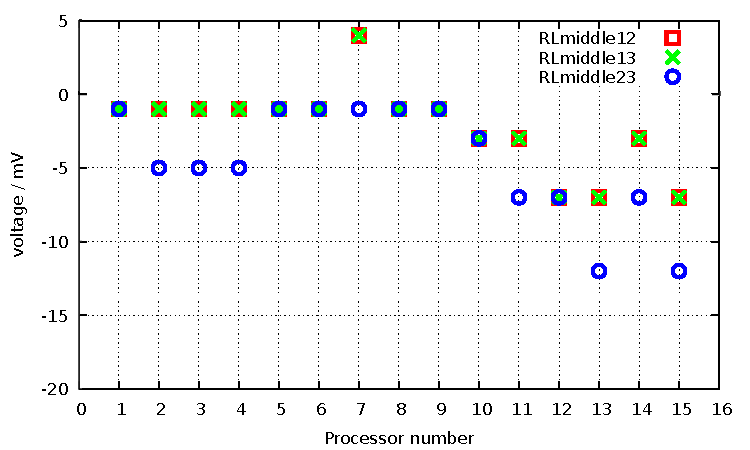
\includegraphics[width=9cm]{../GNU/SelfTMitL.pdf}
    \caption{with \(680\Omega\)}
    \label{fig:SelfTMitL}
  \end{subfigure}
  ~
  \begin{subfigure}[b]{9cm}
    \centering
    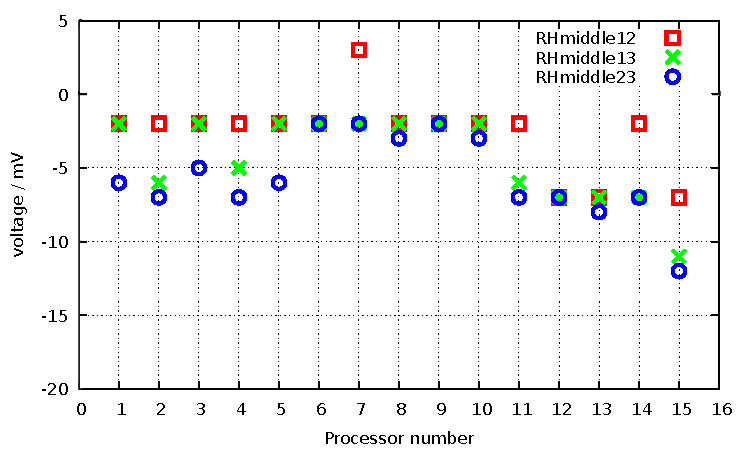
\includegraphics[width=9cm]{../GNU/SelfTMitH.pdf}
    \caption{with \(470k\Omega\)}
    \label{fig:SelfTMitH}
  \end{subfigure}
  \caption{Selftest: difference to ideal mean voltage}
\end{figure}

\begin{figure}[H]
  \begin{subfigure}[b]{9cm}
  \centering
    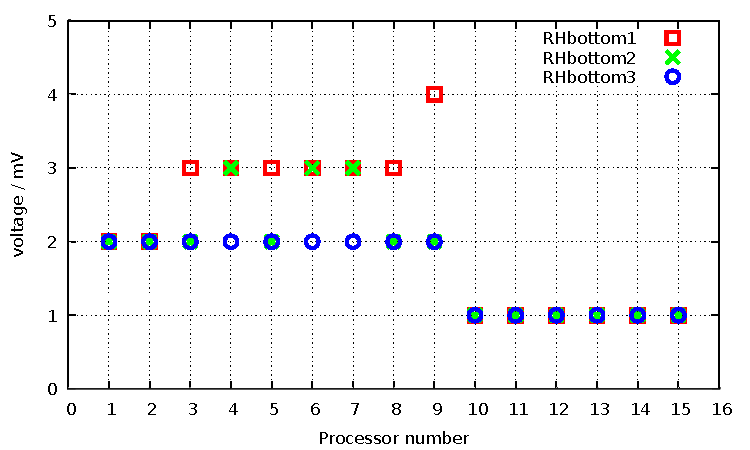
\includegraphics[width=9cm]{../GNU/SelfTbottomH.pdf}
    \caption{with \(470k\Omega\) to 0V}
    \label{fig:SelfTlowH}
  \end{subfigure}
  ~
  \begin{subfigure}[b]{9cm}
  \centering
    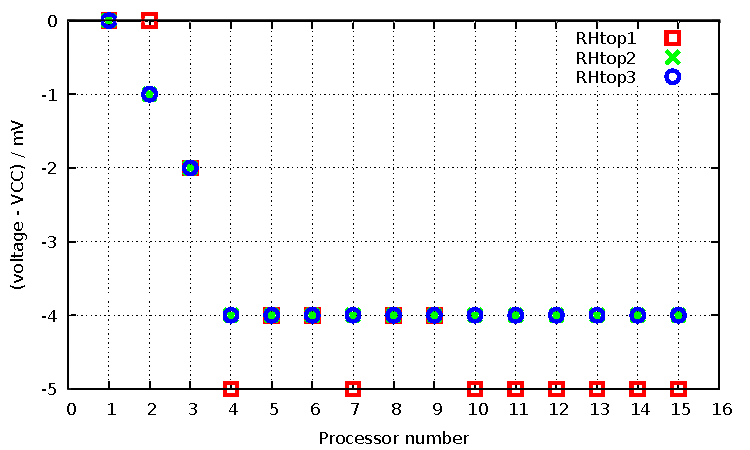
\includegraphics[width=9cm]{../GNU/SelfTtopH.pdf}
    \caption{with \(470k\Omega\) to \(5V\)}
    \label{fig:SelfTtopH}
  \end{subfigure}
  \caption{Selftest: Input voltage}
\end{figure}

\begin{figure}[H]
  \begin{subfigure}[b]{9cm}
  \centering
    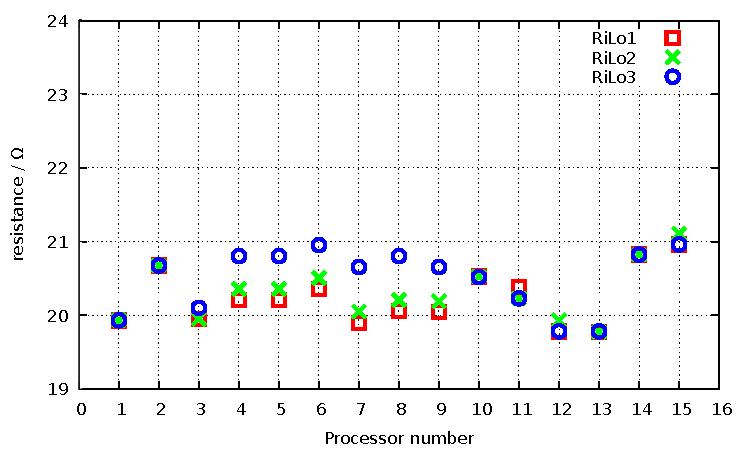
\includegraphics[width=9cm]{../GNU/SelfTRiLo.pdf}
    \caption{with \(680\Omega\) to \(5V\)}
    \label{fig:SelfTRoL}
  \end{subfigure}
  ~
  \begin{subfigure}[b]{9cm}
  \centering
    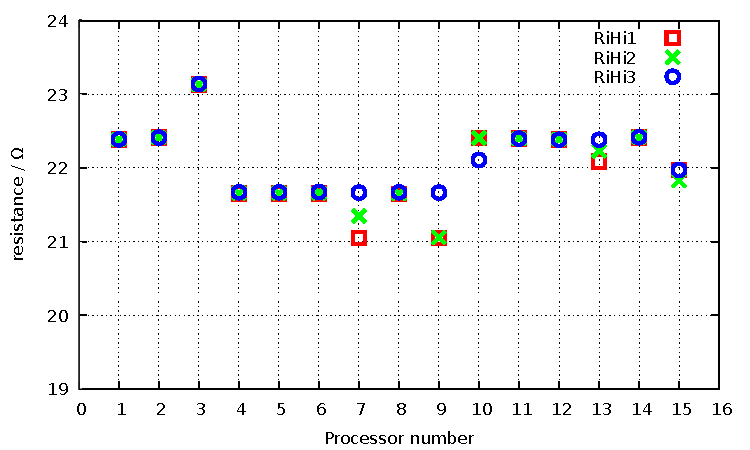
\includegraphics[width=9cm]{../GNU/SelfTRiHi.pdf}
    \caption{with \(680\Omega\) to \(0V\)}
    \label{fig:SelfTRoH}
  \end{subfigure}
  \caption{Selftest: Output resistance}
\end{figure}

\begin{figure}[H]
  \centering
  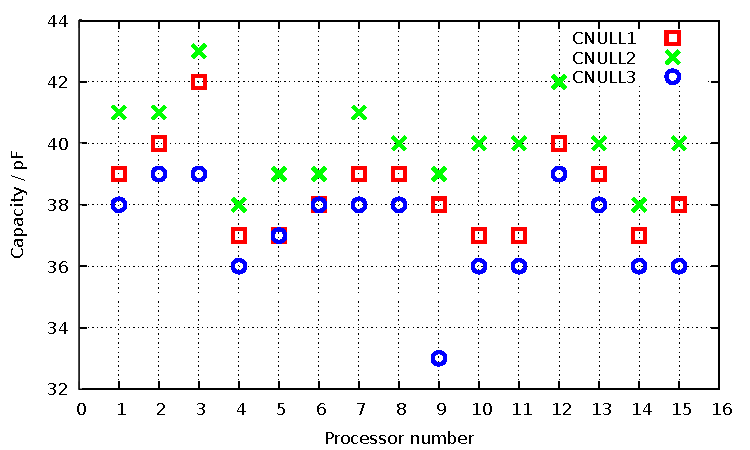
\includegraphics[width=16cm]{../GNU/SelfTcap0.pdf}
  \caption{Selftest: zero offset of the capacity measurement}
  \label{fig:SelfTcap}
\end{figure}

\begin{figure}[H]
  \centering
  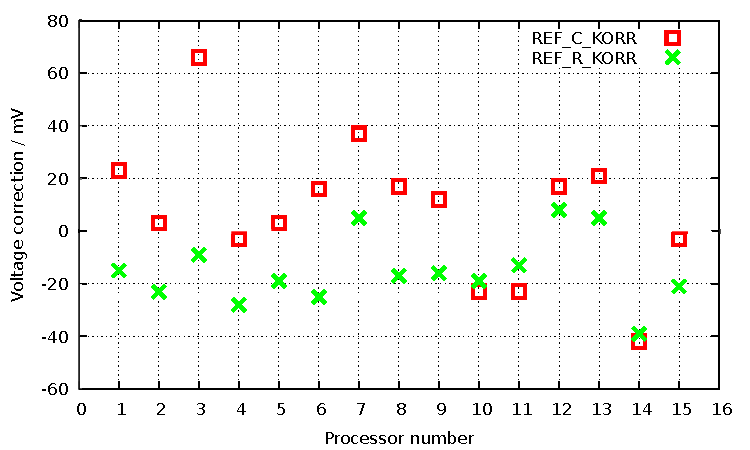
\includegraphics[width=16cm]{../GNU/SelfTrefKorr.pdf}
  \caption{Selftest: correction values after automatic calibration}
  \label{fig:SelfTrefKorr}
\end{figure}

At last I would like to show you the difference voltages of the external at the
AREF pin with a multimeter measured voltages and the internal with the ADC
measured voltages of the reference voltages of 15 different ATmega precessors
and the found correction voltages (REF\_R\_KORR) after the automatic calibration in
figure~\ref{fig:SelfTrefDiff}.
You can see, that the automatic calibration values nearly follow the external measured values.

\begin{figure}[H]
  \centering
  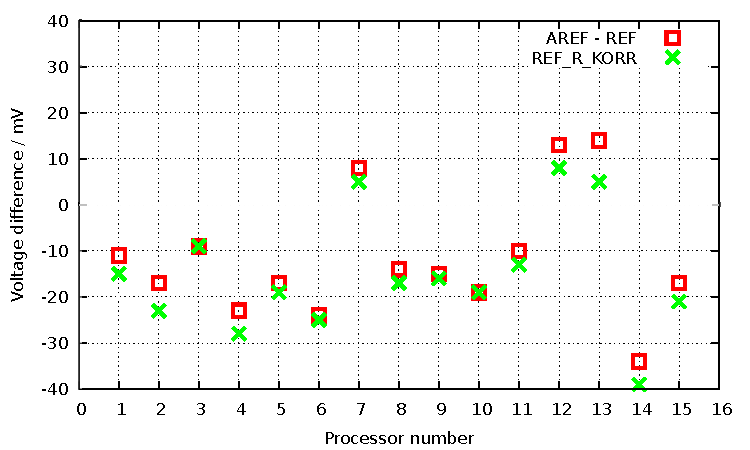
\includegraphics[width=16cm]{../GNU/SelfTrefDiff.pdf}
  \caption{Selftest: Voltage difference of the internal reference}
  \label{fig:SelfTrefDiff}
\end{figure}

